% The first command in your LaTeX source must be the \documentclass command.
\documentclass[sigconf]{acmart}

% \BibTeX command to typeset BibTeX logo in the docs
\AtBeginDocument{%
  \providecommand\BibTeX{{%
    \normalfont B\kern-0.5em{\scshape i\kern-0.25em b}\kern-0.8em\TeX}}}

    
\usepackage{lipsum}
\usepackage{amsfonts}
\usepackage{graphicx}
%\usepackage{epstopdf}
%\usepackage{algorithmic}

%\usepackage{caption}
\usepackage{subcaption}
\captionsetup{compatibility=false}

% Tools for mathematical typesetting
\usepackage{algpseudocode} 
% Typesetting algorithms
\usepackage{algorithm}

\usepackage{amsmath}
%
% ++++ Vectors
\def \vepsilon{ \boldsymbol{\varepsilon} }
\def \vu{ \boldsymbol{u} }
\def \vU{ \boldsymbol{U} }
\def \vzeta{ \boldsymbol{\zeta} }
\def \vx{ \mathbf{x} }
\def \vp{ \boldsymbol{p} }
\def \vs{ \boldsymbol{s} }
\def \vn{ \boldsymbol{n}}
\def \vf{ \boldsymbol{f} }
\def \vxi{\boldsymbol{\xi}}
\def \vom{\boldsymbol{\omega}}

\def \Hx { \hat{1} }
\def \Hy { \hat{2} }
\def \Ht{ \hat{t} }
\def \Hu{ \hat{u} }
\def \Hv{ \hat{v} }
\def \Hw{ \hat{w} }
\def \vc { \boldsymbol{c} }

\def \vn{ \boldsymbol{n} }
\def \vW{ \boldsymbol{W} }
\def \vv{ \mathbf{v} }
\def \vb{ \mathbf{b} }
\def \ve{ \mathbf{e} }
\def \vz{ \mathbf{z} }

\def \vsig{ \boldsymbol{\sigma}}
\def \tnsrsig{ \underset{\thickapprox}{\boldsymbol{\sigma} }}
\def \tnsreps{\underset{\thickapprox}{\boldsymbol{\varepsilon} }}

%  +++++ Tensors
\def \tnsrsig{ \underset{\thickapprox}{\boldsymbol{\sigma} }}
\def \tnsreps{\underset{\thickapprox}{\boldsymbol{\varepsilon} }}
%  +++++ Operators
\def\calB{{\mathcal B}}
\def\calF{{\mathcal F}}
\def\calU{{\mathcal U} }
\def\calUvu{ \mathcal U(\vu) }
\def\calR{\mathcal R }
\def\calS{{ \mathcal S}}
\def\calE{{ \mathcal E}}
\def\calD{{ \mathcal D}}
\def\calP{{ \mathcal P}}
\def\calI{{ \mathcal I}}
\def\calG{{ \mathcal G}}
\def\calL{{ \mathcal L}}

\def \vX{ \mathbf{x} }
\def \vY{ \mathbf{y} }
\def \vg{ \mathbf{g} }
\def \vq {\mathbf{q} }

%**************************************
\newcommand{\alp}[3]{{\left . \alpha_{#1} \right |^{#2}_{#3}\ }}
\newcommand{\bet}[3]{{\left .  \beta_{#1} \right |^{#2}_{#3}\ }}
\newcommand{\Balp}[3]{{\left . \BM {\alpha}_{#1} \right |^{#2}_{#3}\ }}
\newcommand{\Bbet}[3]{{\left . \BM {\beta}_{#1} \right |^{#2}_{#3}\ }}
\newcommand{\Bzet}[2]{{\BM {\zeta}^{#1}_{#2}}}
\newcommand{\B}[1]{{\underline{#1}}}
\newcommand{\Bf}[1]{\boldsymbol{#1}}
\newcommand{\Bc}[1]{\mathcal{#1}}
\newcommand{\Bd}[1]{\mathbb{#1}}
\newcommand{\Bs}[1]{\mathsf{#1}}
\newcommand{\dif}{\mathrm{d}}
\newcommand{\pdif}[2]{\frac{\partial {#1}}{\partial {#2}}}
\newcommand{\pfrac}[2]{\frac{\partial {#1}}{\partial {#2}}}
\newcommand{\scite}[1]{\textsuperscript{\cite{#1}}}
\newcommand{\ul}{\underline}
\newcommand{\II}{\ensuremath{I \hspace{-0.2em} I}}
\newcommand{\III}{\ensuremath{I \hspace{-0.2em} I \hspace{-0.2em} I}}
\newcommand{\CI}{\mathbf{C} \hspace{-0.6em} \mbox{\small I} }
\newcommand{\ci}{\mathbf{c} \hspace{-0.6em} \mbox{\small I} }
\newcommand{\ljump}{\left [  \hspace{-0.21em} \left | }
\newcommand{\rjump}{\right | \hspace{-0.21em} \right ]}
\newcommand{\odif}[2]{\frac{\mathrm{d}  {#1}}{\mathrm{d} {#2}}}
\newcommand{\into}{ \int_{\Omega}}
\newcommand{\difo}{ \;\mathrm{d}\Omega}
\newcommand{\difg}{ \;\mathrm{d}\Gamma}
\newcommand{\BM}[1]{\mbox{\boldmath $#1$}}
\newcommand{\BMB}[1]{\mbox{$\mathbb #1$}}
%\newcommand{\BM}[1]{\mbox{$\mathbf  #1$}}
\newcommand{\bdiff}{\BM{\cal D}}
\newcommand{\diff}{{\cal D}}
\newcommand{\<}{\langle}
\renewcommand{\>}{\rangle}
\newcommand{\Nel}{N_{el}}
\newcommand{\smfrac}[2]{\mbox{$\frac{#1}{#2}$}}


\newcommand{\lon}{\lambda}
\newcommand{\lat}{\theta}
\newcommand{\lond}{\lambda}
\newcommand{\latd}{\theta}
\newcommand{\lons}{\lambda^{\rm e}}
\newcommand{\lats}{\theta^{\rm e}}
\newcommand{\lf}{\left}
\newcommand{\rt}{\right}
\newcommand{\lp}{\lf (}
\newcommand{\rp}{\rt )}
\newcommand{\ep}{\varepsilon}
\newcommand{\tngt}{\boldsymbol{\tau}}
\newcommand{\utngt}{\hat{\boldsymbol{\tau}}}
\newcommand{\unrml}{\hat{\boldsymbol{\eta}}}
\newcommand{\frc}{\mathbf{F}}
\newcommand{\matlab}{\textsc{Matlab\;}}
\newcommand{\inner}[2]{\langle #1,#2 \rangle}

\def \div{D \cdot}
\def \Xd{ X^{\rm d} }
\def \Xs{ X^{\rm s} }
\def \Yd{ Y^{\rm d} }
\def \Ys{ Y^{\rm s} }
\def \vXd{ \boldsymbol{X}^{\rm d} }
\def \vXs{ \boldsymbol{X}^{\rm s} }
\def \ucd{ \vec{\alpha}^X_{\rm d} }
\def \ucdb{ \vec{\alpha}^Y_{\rm d} }
\def \uXd{ \vec{X}_{\rm d}(t) }
\def \uvXd{ \vec{\vX}_{\rm d} }
\def \uvXs{ \vec{\vX}_{\rm s} }
\def \uYd{ \vec{Y}_{\rm d}(t) }
\def \uXs{ \vec{X}_{\rm s}(t) }

% ++++ Vectors.
\def \vepsilon{ \boldsymbol{\varepsilon} }
\def \vu{ \boldsymbol{u} }
\def \vU{ \boldsymbol{U} }
\def \vzeta{ \boldsymbol{\zeta} }
\def \vx{ \boldsymbol{x} }
\def \va{ \boldsymbol{a} }
\def \vy{ \boldsymbol{y} }
\def \vn{ \boldsymbol{n}}
\def \vt{ \boldsymbol{t}}
\def \vf{ \boldsymbol{f} }
%\def \vX{ \boldsymbol{X} }
\def \vc{ \mathbf{c} }
\def \vd{ \mathbf{d} }
\def \vP{ \boldsymbol{P} }
\def \vB{ \boldsymbol{B} }
\def \vp{ \boldsymbol{p} }
\def \vF{ \boldsymbol{F} }

\def \vs{ \mathbf{s}}

\def \Hx { \hat{1} }
\def \Hy { \hat{2} }
\def \Ht{ \hat{t} }
\def \Hu{ \hat{u} }
\def \Hv{ \hat{v} }
\def \Hw{ \hat{w} }
\def \Htau{ \hat{\tau} }
\def \vhtau{ \boldsymbol{\Htau} }
\def \vc { \boldsymbol{c} }
\def \vr { \mathbf{r} }
\def \ve{ \boldsymbol{e} }
\def \vW{ \boldsymbol{W} }
\def \vv{ \mathbf{v} }

\def \vsig{ \boldsymbol{\sigma}}
\def \tnsrsig{ \underset{\thickapprox}{\boldsymbol{\sigma} }}
\def \tnsreps{\underset{\thickapprox}{\boldsymbol{\varepsilon} }}
\newcommand{\calp}{\mathbf{p}}
\newcommand{\Erbf}{E_{\rm rbf}}
\def\bicgstab{{BICGSTAB}} 


% ++++ Vectors.
\def \vepsilon{ \boldsymbol{\varepsilon} }
\def \vu{ \boldsymbol{u} }
\def \vU{ \boldsymbol{U} }
\def \vzeta{ \boldsymbol{\zeta} }
\def \vx{ \boldsymbol{x} }
\def \vn{ \boldsymbol{n}}
\def \vf{ \boldsymbol{f} }
\def \vX{ \boldsymbol{X} }
\def \vZ{ \boldsymbol{Z} }
\def \vXd{ \boldsymbol{X}^{\rm d} }
\def \vXs{ \boldsymbol{X}^{\rm s} }
\def \vY{ \boldsymbol{Y} }
\def \vc{ \boldsymbol{c} }
\def \vP{ \boldsymbol{P} }
\def \vF{ \boldsymbol{F} }

% scalars
\def \Xd{ X^{\rm d} }
\def \Xs{ X^{\rm s} }
\def \Yd{ Y^{\rm d} }
\def \Ys{ Y^{\rm s} }
\def \Zd{ Z^{\rm d} }
\def \Zs{ Z^{\rm s} }

\def \Hx { \hat{1} }
\def \Hy { \hat{2} }
\def \Ht{ \hat{t} }
\def \Hu{ \hat{u} }
\def \Hv{ \hat{v} }
\def \Hw{ \hat{w} }
\def \Htau{ \hat{\tau} }

% Grady's commands
\def \ucd{ \vec{c}^X_{\rm d} }
\def \uXd{ \vec{X}_{\rm d}(t) }
\def \uvXd{ \vec{\vX}_{\rm d} }
\def \uvXs{ \vec{\vX}_{\rm s} }
\def \uYd{ \vec{Y}_{\rm d}(t) }
\def \uXs{ \vec{X}_{\rm s}(t) }
\def \uTd{ \vec{T}_{\rm d} }
\def \uvZd{ \vec{\vZ}_{\rm d} }
\def \uvFs{ \vec{\vF}_{\rm s} }
\def \uvFTs{ \vec{\vF}_{\rm s}^{\rm T} }
\def \uvFBs{ \vec{\vF}_{\rm s}^{\rm B} }
\def \uvFCs{ \vec{\vF}_{\rm s}^{\rm C} }
\def \tngtd{ \tngt_{\rm d} }
\def \utngtd{ \vec{\tngt}_{\rm d} }
\def \uutngtd{ \vec{\hat{\tngt}}_{\rm d} }
\def \utngtslon{ \vec{\tngt}_{\rm s}^{\lon} }
\def \utngtslat{ \vec{\tngt}_{\rm s}^{\lat} }
\def \uunrmls{ \vec{\unrml}_{\rm s} }
\def \Es{ \mathcal{E}_{\rm s} }
\def \ub{ \vec{b}_{\lon} }
\def \ubd{ \ub^{n} }
\def \ubs{ \vec{b}_{\lon,\lat} }
\def \ubsd{ \ubs^{m,n} }
\newcommand{\Dlond}[1]{\mathcal{D}_{\lond}^{#1}}
\newcommand{\Dlons}[1]{\mathcal{D}_{\lons}^{#1}}
\newcommand{\Dlonlatd}[2]{\mathcal{D}_{\lond,\latd}^{#1,#2}}
\newcommand{\Dlonlats}[2]{\mathcal{D}_{\lons,\lats}^{#1,#2}}
\newcommand{\ds}{\displaystyle}
\newcommand{\Sph}{\mathbb{S}^2}

\def \vhtau{ \boldsymbol{\Htau} }
\def \vc { \boldsymbol{c} }
\def \vn{ \boldsymbol{n} }
\def \vW{ \boldsymbol{W} }
\def \vv{ \mathbf{v} }
\def \vsig{ \boldsymbol{\sigma}}
\def \tnsrsig{ \underset{\thickapprox}{\boldsymbol{\sigma} }}
\def \tnsreps{\underset{\thickapprox}{\boldsymbol{\varepsilon} }}

%  +++++ Tensors
\def \tnsrsig{ \underset{\thickapprox}{\boldsymbol{\sigma} }}
\def \tnsreps{\underset{\thickapprox}{\boldsymbol{\varepsilon} }}

%  +++++ Operators
\def\calA{{\mathcal A}}
\def\calB{{\mathcal B}}
\def\calF{{\mathcal F}}
\def\calU{{\mathcal U} }
\def\calUvu{ \mathcal U(\vu) }
\def\calR{\mathcal R }
\def\calS{{ \mathcal S}}
\def\calE{{ \mathcal E}}
\def\calD{{ \mathcal D}}

\newcommand{\Nd}{N_{\rm d}}
\newcommand{\Ns}{N_{\rm s}}
\newcommand{\frcT}{\frc^{\rm T}}
\newcommand{\frcB}{\frc^{\rm B}}
\newcommand{\frcC}{\frc^{\rm C}}
\newcommand{\kt}{k_{\rm t}}
\newcommand{\kb}{k_{\rm b}}
\newcommand{\KC}{K_{\rm C}}
\newcommand{\ellC}{l_{0,\rm C}}

%\let\oldenumerate\enumerate
%\renewcommand{\enumerate}{
%  \oldenumerate
%  \setlength{\itemsep}{1pt}
%  \setlength{\parskip}{0pt}
%  \setlength{\parsep}{0pt}
%}

%\let\olditemize\itemize
%\renewcommand{\itemize}{
%  \olditemize
%  \setlength{\itemsep}{1pt}
%  \setlength{\parskip}{0pt}
%  \setlength{\parsep}{0pt}
%}

% Notation for the augmented RBF system (which is a saddle point)
\newcommand{\Asp}{\widetilde{A}}
\newcommand{\csp}{\widetilde{\vc}}
\newcommand{\fsp}{\widetilde{\vf}}

\newcommand{\comment}[1]{{\color{red}{[#1]}}}
%\ifpdf%
%  \DeclareGraphicsExtensions{.eps,.pdf,.png,.jpg}
%\else
%  \DeclareGraphicsExtensions{.eps}
%\fi
\usepackage{amsopn}
\usepackage{amssymb}
\DeclareMathOperator{\diag}{diag}
\usepackage{booktabs}
\usepackage{float}

\newcommand{\bs}[1]{\ensuremath{\boldsymbol #1}}
\newcommand{\mynote}[3]{
	\textcolor{#2}{\fbox{\bfseries\sffamily\scriptsize#1}}
		{\small$\blacktriangleright$\textsf{\emph{#3}}$\blacktriangleleft$}
}

\newcommand{\mr}[1]{\mynote{Majid}{blue}{#1}}
\newcommand{\hs}[1]{\mynote{Hari}{olive}{#1}}

\renewcommand{\algorithmicrequire}{\textbf{Input:}}
\renewcommand{\algorithmicensure}{\textbf{Output:}}

\newcommand{\mvec}{\textsc{matvec}}
\newcommand{\mm}{\textsc{matmult}}
\newcommand{\recmm}{\textsc{recurs\_matmult}}
\newcommand{\spr}{\textsc{split\_by\_row}}
\newcommand{\spc}{\textsc{split\_by\_col}}
\newcommand{\nnzsz}{\textsc{nnz\_mat\_size}}

% to remove ``PDF inclusion'' warning.
\pdfsuppresswarningpagegroup=1

\iffalse    
% Rights management information. 
% This information is sent to you when you complete the rights form.
% These commands have SAMPLE values in them; it is your responsibility as an author to replace
% the commands and values with those provided to you when you complete the rights form.
%
% These commands are for a PROCEEDINGS abstract or paper.
\copyrightyear{2019}
\acmYear{2019}
\setcopyright{acmlicensed}
\acmConference[ICPP '19]{ICPP '19: ACM Symposium on Neural Gaze Detection}{June 03--05, 2018}{Kyoto, Japan}
\acmBooktitle{Woodstock '18: ACM Symposium on Neural Gaze Detection, June 03--05, 2018, Woodstock, NY}
\acmPrice{15.00}
\acmDOI{10.1145/1122445.1122456}
\acmISBN{978-1-4503-9999-9/18/06}

%
% These commands are for a JOURNAL article.
%\setcopyright{acmcopyright}
%\acmJournal{TOG}
%\acmYear{2018}\acmVolume{37}\acmNumber{4}\acmArticle{111}\acmMonth{8}
%\acmDOI{10.1145/1122445.1122456}

%
% Submission ID. 
% Use this when submitting an article to a sponsored event. You'll receive a unique submission ID from the organizers
% of the event, and this ID should be used as the parameter to this command.
%\acmSubmissionID{123-A56-BU3}

%
% The majority of ACM publications use numbered citations and references. If you are preparing content for an event
% sponsored by ACM SIGGRAPH, you must use the "author year" style of citations and references. Uncommenting
% the next command will enable that style.
%\citestyle{acmauthoryear}
\fi


\begin{document}

%
% The "title" command has an optional parameter, allowing the author to define a "short title" to be used in page headers.
\title[Divide and Conquer Distributed Matrix-Matrix Multiplication]{A Divide and Conquer Distributed Matrix-Matrix Multiplication}

%
% The "author" command and its associated commands are used to define the authors and their affiliations.
% Of note is the shared affiliation of the first two authors, and the "authornote" and "authornotemark" commands
% used to denote shared contribution to the research.
\author{Majid Rasouli}
\email{rasouli@cs.utah.edu}
%\orcid{1234-5678-9012}
%\authornotemark[1]
\affiliation{%
  \institution{School of Computing \\ University of Utah}
  \city{Salt Lake City}
  \state{Utah}
}

\author{Robert M. Kirby}
\email{kirby@cs.utah.edu}
\affiliation{%
  \institution{School of Computing \\ University of Utah}
  \city{Salt Lake City}
  \state{Utah}
}

\author{Hari Sundar}
\email{hari@cs.utah.edu}
\affiliation{%
  \institution{School of Computing \\ University of Utah}
  \city{Salt Lake City}
  \state{Utah}
}

% By default, the full list of authors will be used in the page headers. Often, this list is too long, and will overlap
% other information printed in the page headers. This command allows the author to define a more concise list
% of authors' names for this purpose.
%\renewcommand{\shortauthors}{Majid Rasouli, et al.}

\begin{abstract}
Algebraic Multigrid (AMG) is a popular solver and preconditioner for large sparse linear systems, especially the ones obtained from the discretization of elliptic operators.
A key bottleneck for the scalability of the setup phase of AMG is the Matrix-matrix multiplication (MatMult) required for computing the sparse grid representation. While significant work has been done on optimizing matrix-matrix multiplication, in this work, we optimize it in the context of the matrix multiplications encountered in the setup phase of AMG. Specifically, we designed a new divide and conquer sparse MatMult, that is scalable and makes use of the specific structure of the restriction and prolongation matrices. This combined with an efficient communication pattern during parallel MatMult provides excellent performance for our AMG setup. We compare our solver with PETSc to demonstrate the performance improvements gained using our methods.
\end{abstract}

\keywords{Matrix-Matrix Product, Algebraic Multigrid, AMG, Iterative Solver, Sparse, Preconditioned Conjugate Gradient, Preconditioner}

\iffalse
% A "teaser" image appears between the author and affiliation information and the body 
% of the document, and typically spans the page. 
\begin{teaserfigure}
  \includegraphics[width=\textwidth]{sampleteaser}
  \caption{Seattle Mariners at Spring Training, 2010.}
  \Description{Enjoying the baseball game from the third-base seats. Ichiro Suzuki preparing to bat.}
  \label{fig:teaser}
\end{teaserfigure}
\fi

\maketitle

\section{Introduction}\label{sec:intro} %1page

Chemical transport is a highly interesting phenomenon in a variety of fields like environmental pollutants tracking, biological processes like blood clotting and industrial applications like solvent manufacturing. To study this effectively, we need accurate models that track and predict these chemicals. Many of these applications often involve more than one chemical species which move and interact among themselves. As such, modeling of these processes highly depend on the accuracy with which we can track the interplay between these chemicals. Variation in the chemical population often occurs because of movement and reactions among themselves, thus creating more chemical species or destroying the existing ones. Due to the complex nature of the problem, the advection-diffusion equation shown in \eqref{eqn1} is often used to obtain a numerical approximation of the exact location and population of the chemical species. Here, $D$ referes to the diffusion coefficient and $U$ refer to the flow velocity. It is equally important that we track the accuracy of these models while tracking the chemical species. One of the most common way to ensure accuracy is to compare the numerical solution against the analytical solution. The advection-diffusion equation is being extensively studied and analytically solved for the case of constant diffusion coefficient, with uniform flow \cite{carslaw1959heat,van1982analytical}. However, many naturally occurring processes are more involved than the constant diffusion coefficient or uniform flow can model. One such process is described in the next section.


\begin{align}
    \frac{\partial  \vc}{\partial t} = -U\frac{\partial \vc}{\partial x} + D\frac{\partial^2 \vc}{\partial x^2} \label{eqn1}
\end{align}

\subsection{Variable Diffusion case in Elliptic PDE} \label{sec:Thrombosis}

We now build the model problem of variable diffusion which is an example of elliptic PDE, and motivate the application of multigrid preconditioning methods to numerically solve the resulting equation. Consider the set of equation that arise out of the modeling of chemical transport and interactions resulting from the biological process of blood clotting (specifically, \textit{thrombosis}), popularly knows as the Leiderman-Fogelsen model \cite{leiderman2011grow,l2013influence}.\\

Depending on the roles they play in the process, the interesting quantities of this model can be divided into the following classes: 
\begin{enumerate}
\item Mobile unactivated ($P^{m,u}$), 
\item Mobile activated ($P^{m,a}$), 
\item Platelet-bound activated ($P^{b,a}$)
\item Subendothelium-bound activated ($P^{se,a}$)
\end{enumerate}


\begin{align}
    \frac{\partial P^{m,u}}{\partial t} = \underbrace{-\nabla \cdot \{ W(\phi^T) (\vu P^{m,u} - D \nabla P^{m,u}))\} }_\text{Transport by advection and diffusion} \nonumber\\
    - \underbrace{k_{adh}(\vx) \{P_{max} - P^{se,a} \} P^{m,u}}_\text{Adhesion to subendothelium} \nonumber\\
    - \underbrace{\{A_1 (e_2) +A_2([ADP])\}P^{m,u} }_\text{Activation by thrombin or ADP} \label{eqn2}
\end{align}

\begin{align}
    \frac{\partial P^{m,a}}{\partial t} = - \nabla \cdot \{W(\phi^T)(\vu P^{m,a} - D \nabla P^{m,a} ) \} \nonumber\\
    -k_{adh}(\vx)\{P_{max} - P^{se,a} \} P^{m,a} \nonumber\\
    +\{ A_1 (e_2) + A_2([ADP])P^{m,u} \nonumber\\
    -\underbrace{k_{coh} g(\eta) P_{max} P^{m,a}}_\text{Cohesion to bound platelets}. \label{eqn3}
\end{align}
$k_{adh}(\vx)$ is assumed to  be a positive constant for points $\vx$ within one platelet diameter of subendothelium and zero elsewhere. 

\begin{align} 
    W(\phi^T) = tanh(\pi (1-\phi^T)),  \label{eqn6}
\end{align}
where, $\phi^T = P^{se,a}+P^{b,a}+\frac{P_0}{P_{maxse}}(P^{m,u}+P^{m,a})$, $P_{maxse} and P_{max}$ are a constants for maximum number density for platelets as per \cite{leiderman2011grow}.


In order to numerically solve the model equations of the kind \eqref{eqn2} and \eqref{eqn3}, we need to vary the diffusion coefficient  (depicted by $W(\phi^T)D$) per time-step. The resulting elliptical PDEs can be solved using the Finite Element method. We use the Finite Element software package Nektar++ \cite{nekpp} version 4.4.1 to solve the continuous galerkin problem arising out of the changing diffusion coefficient per time-set. It provides an unsteady diffusion solver that expects the mesh file describing the geometry of the domain and the related solver parameters.\\

While multigrid methods, specifically algebraic multigrid (AMG) methods in conjunction with Krylov methods are very effective in solving equations \eqref{eqn2} and \eqref{eqn3}, the high setup cost associated with AMG makes it less attractive when the operator changes very rapidly (due to varying diffusion coefficient). In this work, we explore different strategies for mitigating the high setup cost, while still retaining the efficiency of multigrid. We find that by performing lazy updates for the AMG preconditioner, we can amortize the high setup costs without adversely affecting the convergence rate. We discribe our methods in the next section \S\ref{sec:method} followed by experiments demonstrating the effectiveness of our approach in \S\ref{sec:results}. Finally, we conclude with directions for future research in \S\ref{sec:conclude}. 

\section{Methods}
\label{sec:methods}

In this section, we present our matrix-matrix multiplication algorithm, the choice of the stop condition for the recursive function and how matrices are being divided to smaller blocks. We then explain how the communication is being done in the distributed fashion to help the recursive function scale better.

%We then explain further modifications to the triple matrix multiplication (\ref{eq:rap}) that are part of the AMG setup process.

\subsection{Matrix-Matrix Multiplication}
\label{sec:matmult}

%\subsubsection{Computation}
%\label{sec:comp}
We design a divide and conquer approach to perform the sparse \mm\ in a node-local fashion. The key idea is to perform simple tasks while recursing, having efficient memory access, and to perform the multiplication for small chunks where the resulting matrix can fit into an appropriate cache. For clarity of presentation, we assume that the data is available locally and discuss it as a serial implementation. Shared memory parallelism is added in a straightforward manner.
%We have implemented \mm~ in a recursive fashion.
%We split the matrices recursively in two ways: split by half based on the matrix size and based on number of nonzeros. First we explain the algorithms performing splitting based on the matrix sizes.

To perform the multiplication
\begin{equation}
    C = A \times B
\end{equation}
we keep splitting the matrices horizontally and vertically (Figure~\ref{fig:split2}) based on row size and column size of $A$, until we can fit the result of the multiplication in a dense matrix.

\begin{figure}[tbh]
 \centering
 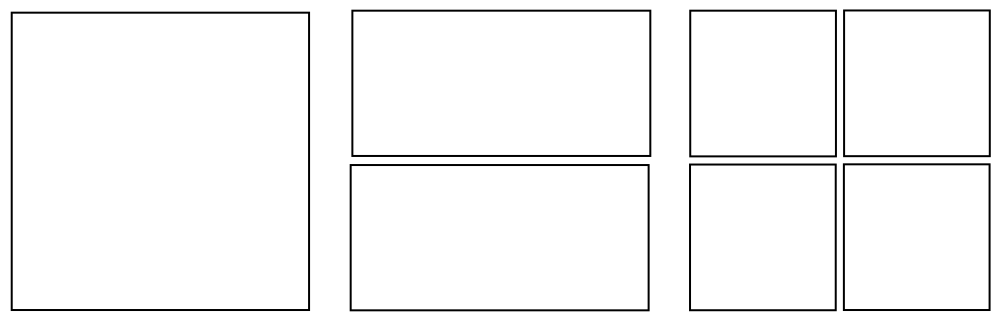
\includegraphics[width=8.5cm,height=2.7cm]{./figures/split2.pdf}
 \caption{A basic scheme that shows splitting the matrix first horizontally, then vertically.}
 \label{fig:split2}
 \Description{}
\end{figure}

The recursive function, \recmm, includes three cases:
\begin{enumerate}
 \item Case 1: Stop the recursion: perform the multiplication.
 \item Case 2: $A$ is horizontal. Split $A$ and $B$.
 \item Case 3: $A$ is vertical. Split $A$ and $B$.
\end{enumerate}

\subsubsection{Case 1}
\label{sec:case1}
First we discuss when we decide to stop the recursive function.  
Our goal is to fit the multiplication result of blocks of $A$ and $B$ in a dense buffer. We show the blocks of $A$ and $B$ as $A_{ij}$ and $B_{lk}$. We use two indices here because matrices gets divided both horizontally and vertically. The size of the dense buffer to store $A_{ij} \times B_{lk}$ is
\begin{equation}
    row\ size\ of\ A_{ij} \times column\ size\ of\ B_{lk}\label{eq:thres}
\end{equation}

Therefore, the obvious choice to decide when to stop the recursion is Equation~ \eqref{eq:thres}, but Figure~\ref{fig:thres} shows why that is not a good choice. If we use Equation~ \eqref{eq:thres} for this example, the splitting process for the top two blocks of the matrix stops at the same step, but the top left block should be divided to more blocks than the top right block.

\begin{figure}[tbh]
 \centering
 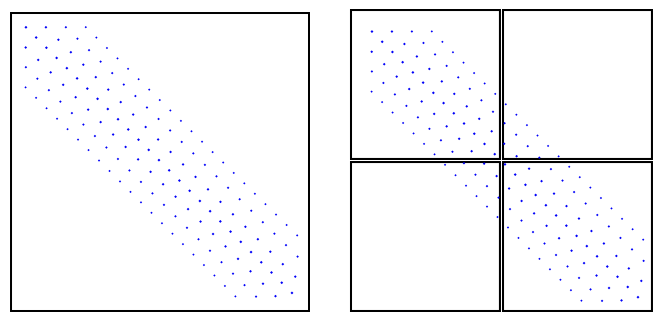
\includegraphics[width=8.5cm,height=4cm]{./figures/split3.pdf}
 \caption{Using row and column sizes to decide when to stop the recursion is not efficient, because the top left block is the same size as the top right one, but it should be divided to more sub-blocks.}
 \label{fig:thres}
 \Description{}
\end{figure}

Furthermore, by splitting sparse matrices recursively, we will have more and more zero rows and columns in the resulting blocks. So, using row size and column size of the blocks is not very helpful. Instead, we use nonzero rows and nonzero columns.

At the start of the recursive function, the number of nonzero rows of A ($A\_nnz\_row$) and nonzero columns of B ($B\_nnz\_col$) are being computed. A threshold for 
\begin{equation}
    \nnzsz = A\_nnz\_row \times B\_nnz\_col
\end{equation}

is set. Our algorithm has a profiling step where it empirically determines the appropriate threshold by running several test cases. On the machines we used,  $20M$ was chosen as the threshold. We continue splitting the matrices until the threshold is reached, and then we preform the multiplication.

%First method uses a dense matrix.
%The matrices are ordered as column-major.
% In the first method, a dense matrix of size $\nnzsz$ is initialized to $0$. \mr{explain better:}Each nonzero of $B$ is multiplied by its corresponding nonzero of $A$ and the result will be added to the corresponding index in the dense matrix. At the end, we go through the dense matrix and add the nonzeros to the final multiplication matrix.

We have implemented two methods to perform the multiplication: 
\begin{enumerate}
    \item dense buffer
    \item hashmap
\end{enumerate}

When performing the multiplication, at least one of the matrices, typically the output, needs random access as it is accumulating the results. Given that the divide and conquer approach has reduced the size of the output matrix, the first approach is to keep a temporary buffer for dense matrix storage. Each nonzero of $B$ is multiplied by its corresponding nonzero of $A$ and the result will be added to the corresponding index in the dense matrix. As long as the dense matrix is small enough to fit within the L2 cache, we should get good performance. At the end of the multiplication, we traverse the dense matrix and extract the non-zeros as a sparse matrix. This approach works well as long as the resulting matrix is dense. We allocate a memory block of size of the threshold before starting the matrix product. When we reach the stop condition for each recursive call, we preform the following steps:
\begin{enumerate}
    \item Initialize the first \nnzsz~ entries to 0.
    \item Perform the multiplication and add the result entries to the buffer matrix.
    \item Extract nonzeros from the dense matrix and add them to C.
\end{enumerate}

When the ratio of nonzeros to \nnzsz~ is low, it becomes inefficient to traverse the whole dense matrix and check for nonzeros in the final stage. To solve this issue, we use an efficient hashmap to achieve similar results without the $\mathcal{O}(n^2)$ overhead of extracting the non-zeros from the dense matrix. The entry's index is the key and its value is the hashmap's value. When we want to add the multiplication of nonzeros of $A$ and $B$ to the hashmap, we check if the index exists in the map. If it exists the value is being added to the existing one's. Otherwise a new entry will be added to the hashmap. Clearly, there is an overhead to this approach that needs to be balanced against the overheads associated with the dense representation. 

To measure of the effectiveness of our method in a practical situation, we have implemented the \recmm~ function in our Algebraic Multigrid solver, called \textit{Saena}, and performed \mm~ twice to compute the coarse matrix based on the 3D Poisson Problem.

In Figure~\ref{fig:lap60}, we compare the two methods for computing coarse matrix $Ac = R \times A \times P$, in which $A$ is the 3D Poisson problem of size $216k$. For $0 \leq \nnzsz \leq 10M$, in $1M$ steps, we compare the two methods in order to develop an efficient hybrid algorithm. For instance, the first point indicates that the dense structure is better than the hashmap approach in $1245$ cases for the multiplications such that $0 \le\ \nnzsz < 1M$. For the lower range the dense representation is better and for the higher range the hashmap is significantly faster. Figure~\ref{fig:eco} shows the same experiment for matrix ID $1882$ from SuiteSparse (Florida) Matrix Collection, which is a sparse matrix of size $1M$ and $5M$ nonzero.

\begin{figure}[tbh]
 \centering
 %\Description{Description}
 \includegraphics[width=8.5cm,height=4cm]{./figures/lap60_range.pdf}
 \caption{Comparison between dense structure method with hashmap to compute coarse matrix $Ac = R \times A \times P$, in which $A$ is the 3D Poisson problem of size $216k$. The plot shows the number of times each method is faster than the other one in intervals of $1M$ for $\nnzsz$.}
 \label{fig:lap60}
 \Description{}
\end{figure}

A combination of these two methods would give us the best performance across different matrix structures and densities. The dense method is being used for the lower range and the hashmap for the higher range.
We have done a series of experiments to determine the threshold when to switch between the two methods. Figures~\ref{fig:lap60} and \ref{fig:eco} suggest to use the dense structure method when $0 \le\ \nnzsz < 4M$ and use hashmap for the rest. We noticed that when hashmaps are better, the difference time between the two methods on average is higher. In other words, on average, $n$ times performing hashmap is faster than $n$ times using the dense structure. So empirically, we found $1M$ to be a good estimate for switching between the two methods.

\begin{figure}[tbh]
 \centering
%\Description{Description}
 \includegraphics[width=8.5cm,height=4cm]{./figures/eco_range.pdf}
 \caption{Comparison between dense structure method with hashmap to compute coarse matrix $Ac = R \times A \times P$, in which $A$ is matrix ID $1882$ from SuiteSparse (Florida) Matrix Collection. The plot shows the number of times each method is faster than the other one in intervals of $1M$ for $\nnzsz$.}
 \label{fig:eco}
 \Description{}
\end{figure}

\begin{figure}[tbh]
 \centering
 %\Description{Description}
 \includegraphics[width=8.5cm,height=5cm]{./figures/mix.pdf}
 \caption{Comparison between the three methods to do Case 1: only using hashmap, only using the dense structure, and the hybrid method. They are used as Case 1 to compute the first coarse matrix (the triple multiplication) on 7 matrices (3D Poisson) of different sizes.}
 \label{fig:mix}
 \Description{}
\end{figure}

Figure~\ref{fig:mix} compares the hybrid method with the basic two methods. We have compared the three approaches on different sizes of 3D Poisson problem, ranging from $8k$ to almost half a million. For instance, for the case where the matrix is of size $512k$, performing the triple matrix product takes $291s$ if only hashmap is used for Case 1, takes $72s$ if only the dense structure is used and finally takes almost $17s$ when the hybrid approach is utilized.


\subsubsection{Case 2}
\label{sec:case2}
When A is horizontal, i.e. its row size is less than or equal to its column size, we halve A by column based on its column size (Figure~\ref{fig:case2_left}). Since row size of B equals column size of A, we halve B by row, so it will be a split similar to A, but horizontally.
Then, the \recmm~ will be called twice, once on $A1$ and $B1$, and again on $A2$ and $B2$ (Algorithm~\ref{alg:case2}). The results of the two multiplications need to be added together at the end. It means, there will be entries for the result matrix with the same index. We call these entries \textit{duplicates}. Since there will be numerous nested recursive calls, we avoid doing adding duplicates at this stage. After the first recursive function is finished, we will perform a sorting and then add the duplicates only once at the end.

\begin{figure}[tbh]
    \centering
    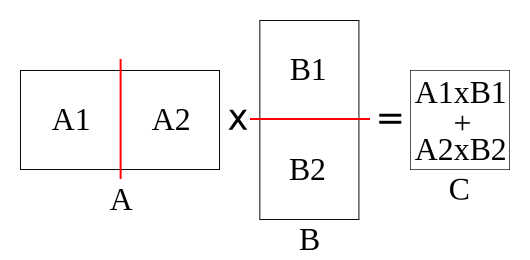
\includegraphics[width=4.5cm,height=2.3cm]{./figures/case2_001.pdf}
    \caption{Case 2: When A is horizontal, split A by column and B by row. Call the recursive function twice.}
    \label{fig:case2_left}
    \Description{}
\end{figure}

\begin{figure}[tbh]
    \centering
    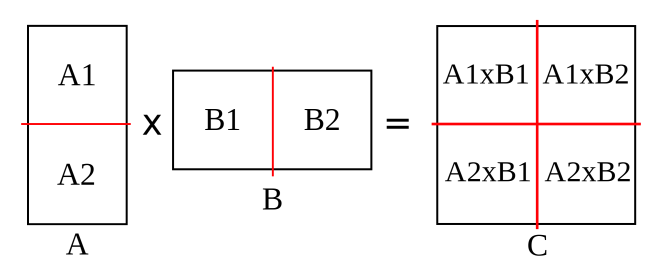
\includegraphics[width=5.5cm,height=2.3cm]{./figures/case3_001.pdf}
    \caption{Case 3: When A is vertical, split A by row and B by column. Call the recursive function four times.}
    \label{fig:case3}
    \Description{}
\end{figure}

\begin{algorithm}[tbh] 
  %\footnotesize
  \caption{Case 2: $C = \recmm2(A, B)$} 
  \begin{algorithmic}[1]
    \Require $A$, $B$
    \Ensure  $C$
    \State $(A1, A2) = \spc(A)$
    \State $(B1, B2) = \spr(B)$
    \State $C \leftarrow \recmm(A1,B1)$
    \State $C \leftarrow \recmm(A2,B2)$
    %\State $C \leftarrow \textsc{mergesort}(C1, C2)$
  \end{algorithmic}
  \label{alg:case2}
  \Description{}
\end{algorithm}

\subsubsection{Case 3}
\label{sec:case3}
When A is vertical, i.e. its row size is greater than its column size, we halve A by row based on its row size and halve B by column (Figure~\ref{fig:case3}). In contrary to the previous case, the column size of B is not related to row size of A, so they are split independently. This time the \recmm~ will be called four times (Algorithm~\ref{alg:case3}).  Although we have 4 recursive calls in this case, but there is no duplicates at the end, which makes this case more efficient than Case 2 for the total time, because it is faster to do the sorting and adding duplicates at the end on a smaller set of entries. 

\iffalse
\begin{figure}[tbh]
 \centering
 %\Description{Description}
 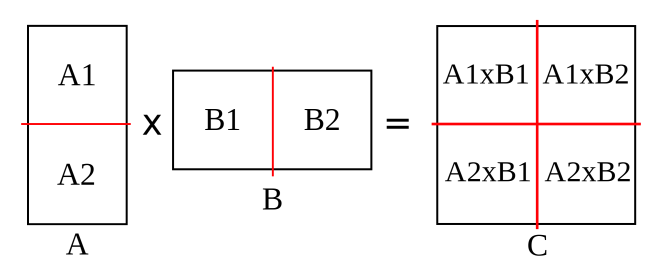
\includegraphics[width=6cm,height=2.5cm]{./figures/case3_001.pdf}
 \caption{Case 3: When A is vertical, split A by row and B by column. Call the recursive function four times.}
 \label{fig:case3}
\end{figure}
\fi

\begin{algorithm}[H] 
  %\footnotesize
  \caption{Case 3: $C = \recmm3(A, B)$} \label{alg:case3} 
  \begin{algorithmic}[1]
    \Require $A$, $B$
    \Ensure  $C$
    \State $(A1, A2) = \spr(A)$
    \State $(B1, B2) = \spc(B)$
    \State $C \leftarrow \recmm(A1,B1)$
    \State $C \leftarrow \recmm(A2,B1)$
    \State $C \leftarrow \recmm(A1,B2)$
    \State $C \leftarrow \recmm(A2,B2)$
    %\State $\textsc{sort}(C)$
  \end{algorithmic}
  \label{alg:case3}
\end{algorithm}

We have also implemented splitting based on the number of nonzeros. In \textit{Case 2}, we split $A$ in a way to have half of nonzeros in $A1$, and the other half in $A2$. The same split is used for $B$. In \textit{Case 3}, we do the same, but separately for both $A$ and $B$. After a series of experiments we noticed that the splitting method based on size scales better than splitting based on nonzeros.

\subsubsection{All together}

When all three cases work together, we have Case 2 and Case 3, that aim to divide the matrices into skinny matrices such that the resulting matrix is small. Then by using a hybrid multiplication algorithm, we get these results. These results are then accumulated and merged together. From a memory access perspective, the accumulation and merging required for Case 2 and 3 is structured access to the matrix, with the only random access happening during Case 1. This makes the overall algorithm very efficient. 

\subsection{Communication}
\label{sec:amg}

In the previous section we explained how to perform \mm~ if the data is available locally. In this section, we explain how the communication is done to perform
\begin{equation}
    C = A \times B
\end{equation}
in a distributed fashion for general (non necessarily symmetric) matrices $A$ and $B$. Also, we show how to improve performance and scalability if $B$ is symmetric.

Matrices are partitioned across multiple processors by row blocks (Figure~\ref{fig:partition}). Since matrices $A$ and $B$ may have different number of rows, they may not be partitioned the same way. To avoid any communication at the end of the multiplication, we avoid communicating $A$ and only communicate $B$. 

\begin{figure}[tbh]
 \centering
 %\Description{Description}
 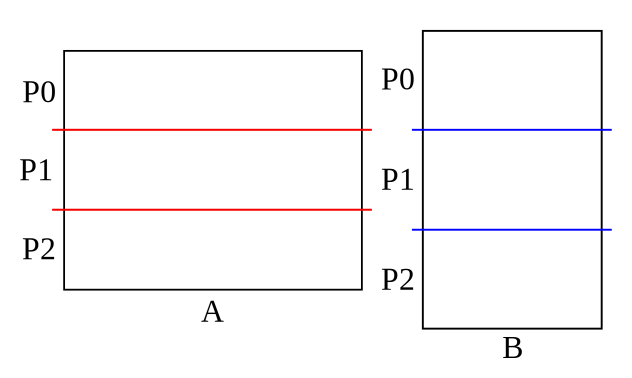
\includegraphics[width=5.3cm,height=2.8cm]{./figures/partition2.pdf}
 \caption{Partitioning of the matrices across the processors in row blocks.}
 \label{fig:partition}
 \Description{}
\end{figure}

\begin{algorithm}[H] 
  %\footnotesize
  \caption{Part 1: $C_i = A_i \times B$}
  \begin{algorithmic}[1]
    \Require $A_i$, $B$
    \Ensure  $C_i$ (result of $A_i \times B$)
    \State $B\_send \leftarrow$ transpose of $R_i$ (locally)
    \For{$k=myrank:myrank+nprocs$}
      \State $R2 \leftarrow\ Irecv(transpose\ of\ R block)\ from\ right\ neighbor$
      \State $Isend(R1)\ to\ left\ neighbor$
      \State $B_{ik} \leftarrow \recmm(A_i, R1)$ 
      \State $wait\ for\ Isend\ and\ Irecv\ to\ finish$
      \State $swap(R1,R2)$
    \EndFor
    \State locally sort $B_i$ and add duplicates
  \end{algorithmic}
  \label{alg:comm1} 
\end{algorithm}

Now, we explain how to compute $B := A \times P$. We assume the same partition of rows of $A$ on also its columns (red lines) since $A$ is square. For columns of $P$ we use the partition of rows of $R$ (blue lines in Figure~\ref{fig:part1b}).
Without loss of generality, let us focus on how to perform \mm ~on processor $P1$. To compute entry $B(i, j)$, we need to multiply row $i$ of $A$ with column $j$ of $P$ and add them together (since we are working with sparse matrices, we only consider the nonzeros here).

\begin{figure}[tbh]
    \centering
    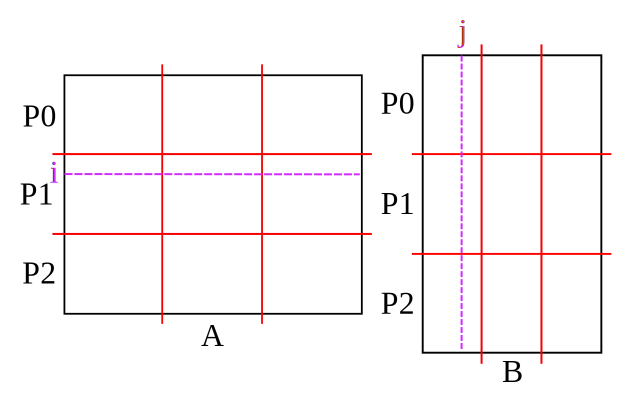
\includegraphics[width=5cm,height=3cm]{./figures/partition3.pdf}
    \caption{Column $j$ of $B$ is stored on different processors.}
    \label{fig:part1b}
    \Description{}
\end{figure}

\begin{figure}[tbh]
    \centering
    \includegraphics[width=5cm,height=2.9cm]{./figures/part1c.pdf}
    \caption{This figure shows how row blocks of $R$ are transpose of column blocks of $P$.}
    \label{fig:part1c}
    \Description{}
\end{figure}

Column $j$ of $P$ is distributed between all the processors. Therefore we need to communicate all nonzeros of that column and then perform $B_{ij} = \sum_{k} A_{ik} P_{kj}$. Since that can lead to significant communication, we make use of the fact that $R$ is the transpose of $P$ and is already available locally because of the multigrid hierarchy. We note that column blocks of $P$ (e.g. $r0$ in Figure~\ref{fig:part1c}) are actually row blocks of $R$ transposed ($rt0$, which is transpose of $r0$).

We have implemented this part in an overlapped fashion; first we do the send and receive commands (to communicate $rt$ blocks) and while this communication is being done, we perform \mm, so saving time for the communication (Algorithm \ref{alg:comm2}). $B_{i}$ in the algorithm is the row block of matrix $B$ on processor $i$ and $B_{ik}$ is the sub-block result of multiplying $A_i$ with $rt_k$.

\begin{algorithm}[H] 
  %\footnotesize
  \caption{Part 1: $B_i = A_i \times P$}
  \begin{algorithmic}[1]
    \Require $A_i$, $R$
    \Ensure  $B_i$ (result of $A_i \times P$)
    \State $R1 \leftarrow$ transpose of $R_i$ (locally)
    \For{$k=myrank:myrank+nprocs$}
      \State $R2 \leftarrow\ Irecv(transpose\ of\ R block)\ from\ right\ neighbor$
      \State $Isend(R1)\ to\ left\ neighbor$
      \State $B_{ik} \leftarrow \recmm(A_i, R1)$ 
      \State $wait\ for\ Isend\ and\ Irecv\ to\ finish$
      \State $swap(R1,R2)$
    \EndFor
    \State locally sort $B_i$ and add duplicates
  \end{algorithmic}
  \label{alg:comm2}
\end{algorithm}

\section{Numerical Results}
\label{sec:results} %2.5 pages

\subsection{Experimental Setup}

All experiments were conducted on a 12-node cluster at the Center for High Performance Computing (CHPC) at 
the University of Utah. Each node consists of a dual-socket Intel Xeon Haswell processors with 14 cores each 
for a total of 28 cores and 128GB per node. 

%The lazy-updates experiments have been done on Chiron servers in \textit{SCI - University of Utah}.
%They are performed using a 64 cores Intel Xeon x7560 2.27GHz (128 with HT) machine with 504GB of RAM and with OS openSUSE 42.1.
% The weak and strong scaling experiments are measured on Kingspeak servers located in \textit{CHPC - University of Utah}. Each node has two sockets, with 14 cores on each socket.

Two sets of experiments have been done for this section. The first experiment shows how lazy-update for AMG behaves on a matrix
generated from a 2D mesh in \textit{Nektar++} which is shown in Figure \ref{fig:mesh}. The mesh has order 7 and has triangles and
quads and is a challenging mesh for AMG. The generated matrix is of size 870 by 870 and has 33761 nonzeros.

The AMG hierarchy is created on an initial matrix $A$. Then the linear system 
$Ax = b$ is solved and number of vcycle iterations that it takes for the solve phase is written on the plot.
Then, the difusion coefficients change based on a sine function to generate another matrix ($B_1$) which is slightly 
different from the initial one. The number of iterations to solve the system $B_1x = b$ is shown on the plot.
The same process is repeated for multiple matrices.

The second set of experiments shows weak scaling and strong scaling of AMG as a preconditioner on 2D Poisson problem.
One MPI task is assigned to each socket, so each node has two MPI tasks, corresponding to our hardware confguration. 
%(except the first one, which has one MPI task in total).
The number of OpenMP threads on each socket is 14.
For the weak scaling each processor has almost 262k degree of freedom. In the strong scaling the total degree of freedom for all
the experiments is $1048000$.

\begin{figure}[H]
 \centering
 \includegraphics[width=8cm,height=7cm]{./figures/mesh.png}
 \caption{The mesh that is used for the sinusoidal diffusion coefficient change experiment.}
 \label{fig:mesh}
\end{figure}

\subsection{Results}

Figure~\ref{fig:strategy1} shows the lazy-update AMG using the first strategy.
The blue and red lines show how the coefficients are generated based on a sine function to create new matrices $B_i$.
By using strategy1, only $As[1]$ of the whole AMG hierarchy will be updated to solve each new linear system $B_ix = b$.
The plot shows that by saving the time using the same AMG hierarchy from the initial matrix, only a couple more (at most 6)
iterations is required to solve a linear system similar to the initial one. So, even though we need to spend a little more
time in the solve phase, almost the entire setup phase can be avoided.

Figure~\ref{fig:strategy2} shows a similar result for the second strategy. Here, all $As$ are updated in the setup phase
for the new matrices, so more setup time comparing to the first strategy is required, but at most 4 additional iterations are required during the solve phase.

\begin{figure}[H]
 \centering
 \includegraphics[width=10cm,height=5cm]{./figures/update2-3.png}
 \caption{Strategy1: The entire AMG hierarchy is re-used without incurring the cost of additional setup, except for the fine matrix. $As[1]$ is the only part that gets updated.
          The orange marks show how many iterations is required to achieve $10^{-12}$ relative tolerance.
          Each orange triangle corresponds to the number of iterations required to solve the system for a new updated matrix.
          The blue (red) triangles are the maximum (minimum) diffusion coefficients used to generate the new matrices.}
 \label{fig:strategy1}
\end{figure}

\begin{figure}[H]
 \centering
 \includegraphics[width=10cm,height=5cm]{./figures/update3-3.png}
 \caption{Strategy2: The aggregations is not updated, but the coarse grid matrices are recomputed. 
 All $As$ matrices get updated, but $Ps$ and $Rs$ are used from the initial AMG hierarchy.
          The orange marks show how many iterations is required to achieve $10^{-12}$ relative tolerance.
          Each orange triangle corresponds to the number of iterations required to solve the system for a new updated matrix.
          The blue (red) triangles are the maximum (minimum) diffusion coefficients used to generate the new matrices.}
 \label{fig:strategy2}
\end{figure}

Figure \ref{fig:solvesetup} shows the weak and strong scalability of the solve and setup phases,
for the 2D Poisson problem. One can easily notice that the setup time takes more than 17 times more time than the setup phase for this experiment.
From that, it is obvious why we accept a small increase in the solve time, to avoid doing some steps of the setup phase in the strategies we discussed.

\begin{figure}[H]
 \centering
 \includegraphics[width=13cm,height=5cm]{./figures/solvesetup.png}
 \caption{strong (blue) and weak scaling (orange) of the AMG solve (left) and setup (right) phases.
          The setup phase takes significantly more time than the solve step.}
 \label{fig:solvesetup}
\end{figure}


\newpage
\bibliographystyle{ACM-Reference-Format}
\bibliography{ref}

\end{document}
